\section{体感速度モデルの提案}
これまで、スケールスピードと実速度を比較することで、体感速度はスケールスピードと一致せず、単なるスケール比に一致することが明らかになった。
さらに、その過程において体感速度を変化させるパラメータを発見した。列挙した中で最も影響力のあるパラメータが、走行映像のクロップ率やカメラの画角・ドライバの視野角であることが明らかになった。
そこで、走行映像のクロップ率とドライバの視野角を体感速度変化のパラメータとして、体感速度を定式化する手法を提案する。本研究では、実測値との比較として、視野角・ディスプレイ比等、DS環境におけるパラメータを定数とした
幾何学計算による幾何学モデルを提案する。

\subsection{原理}
実車が同じ速度で走行する場合でも、視野角が広い方が、体感速度が速く感じるという現象が生じる基準視野角と、ある視野角での画面上の一方から他方の点にかけてのピクセルの移動距離の比が体感速度の比となる。
図\ref{taikan:pixel}に、ピクセルの移動距離の考え方を示す。
同様の原理として、交通事故で取り上げられるコリジョンコース現象が挙げられる。複数の走行映像において、ピクセルの移動速度が一致する時、体感速度の比と一致していることが望ましい。

\begin{figure}[h]
  \begin{center}
  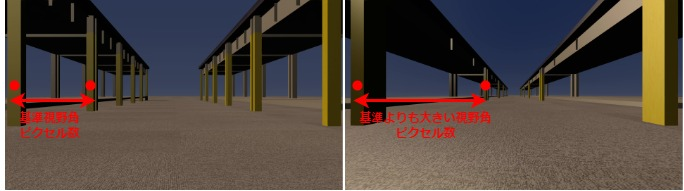
\includegraphics[width=.65\linewidth]{img/11.jpg}
  \caption{ピクセルの移動距離の考え方}
  \label{taikan:pixel}
  \end{center}
\end{figure}

\clearpage
\subsection{体感速度モデルの定式化}
体感速度を求めるために、映像中のポール間の移動の際に映像中の移動ピクセル数と、環境によって決まるパラメータを定式化する。
ここでは、体感速度$v_{sense}$を、視野角の関数$f(h_{fov_v})$で表し、$h_{fov_v}$を、クロップ率の関数$g(n)$で表すことを目標とする。
実際の速度\verb|(実速度とする)|を$v_2$とすると、式\eqref{taikan:eq:model1}、\eqref{taikan:eq:model2}に示す関係式を求める。

\begin{align}
  v_{sense} = f(h_{fov_v})\cdot v_s = f(g(n))\cdot v_s \label{taikan:eq:model1}\\
  h_{fov_v} = g(n) \label{taikan:eq:model2}
\end{align}

まず、ディスプレイのアスペクト比とサイズ(ディスプレイの対角線の長さ)をディスプレイの縦・横の長さに変換する式を式\eqref{taikan:eq:dis1}、\eqref{taikan:eq:dis2}に示す。図\ref{taikan:displaytosize}
にディスプレイ長さの概要と諸条件を示す。

\begin{figure}[h]
  \begin{center}
  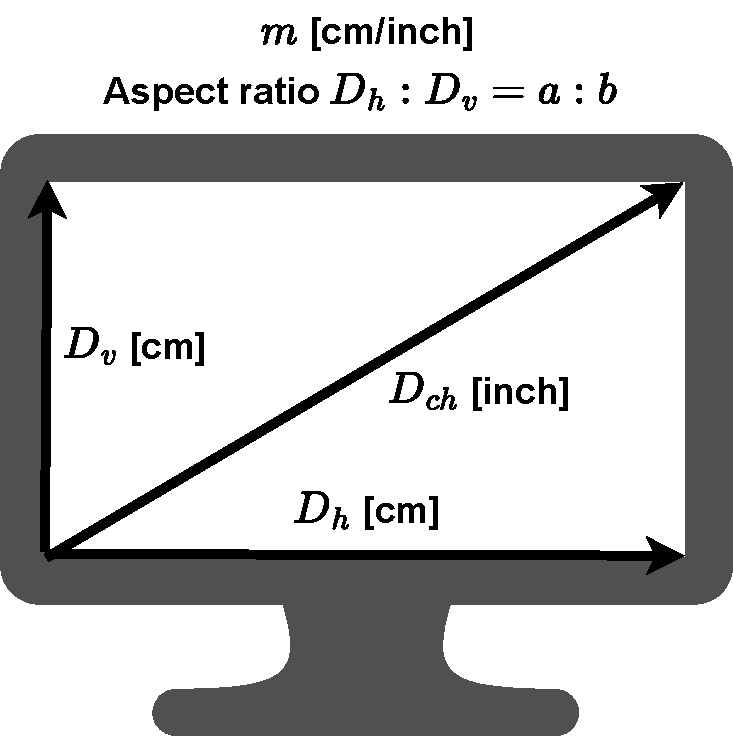
\includegraphics[width=.65\linewidth]{img/12.pdf}
  \caption{ディスプレイ長さの概要と諸条件}
  \label{taikan:displaytosize}
  \end{center}
\end{figure}

\begin{align}
    D_v = D_{ch} \cdot m \cdot \frac{b}{\sqrt{a^2+b^2}} \label{taikan:eq:dis1}\\
    D_h = D_{ch} \cdot m \cdot \frac{a}{\sqrt{a^2+b^2}} \label{taikan:eq:dis2}
\end{align}

$D_v$:ディスプレイの縦の長さ\si{[cm]}、$D_h$:ディスプレイの横の長さ\si{[cm]}、$D_{ch}$:ディスプレイの対角線の長さ\si{[inch]}、
$m$:2.4\si{[cm/inch]}、$a$:ディスプレイの横のアスペクト比:16、$b$:ディスプレイの縦のアスペクト比:9とする。

次に、ディスプレイの縦・横の長さとディスプレイとの視点距離をDS上での水平・垂直方向の基準視野角に式\eqref{taikan:eq:kijun1}、\eqref{taikan:eq:kijun2}を用いて変換する。
図\ref{taikan:kijuntods}に基準視野角とその導出の諸条件を示す。


\begin{figure}[h]
  \begin{center}
  \subfigure[水平方向]{
  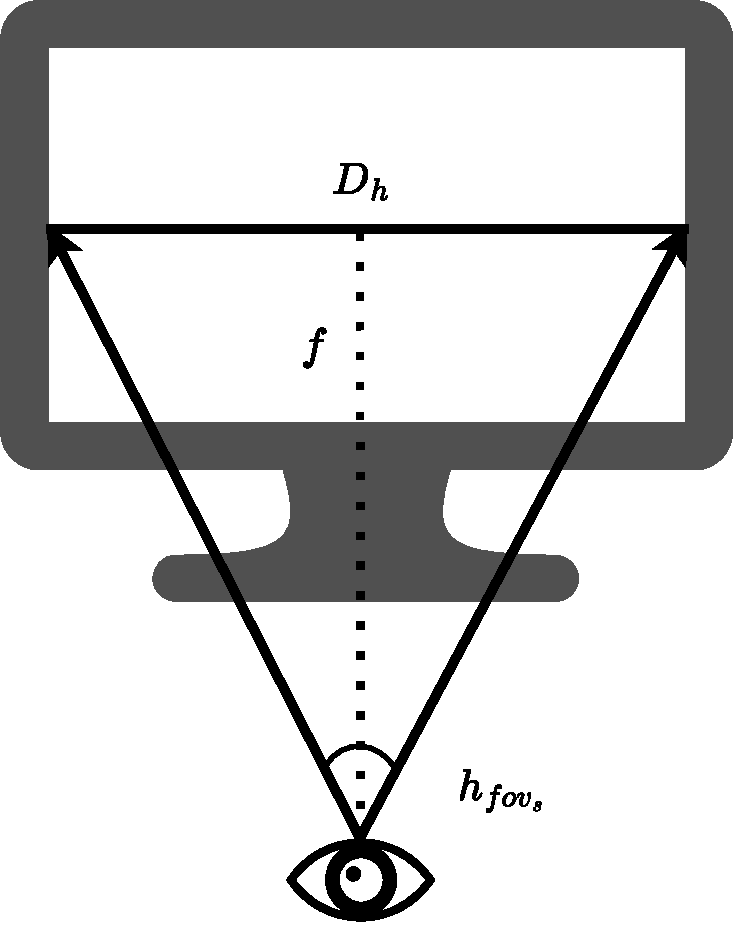
\includegraphics[width=.4\columnwidth]{img/13_1.pdf}
  \label{taikan:kijuntods1}
  }
  \subfigure[垂直方向]{
  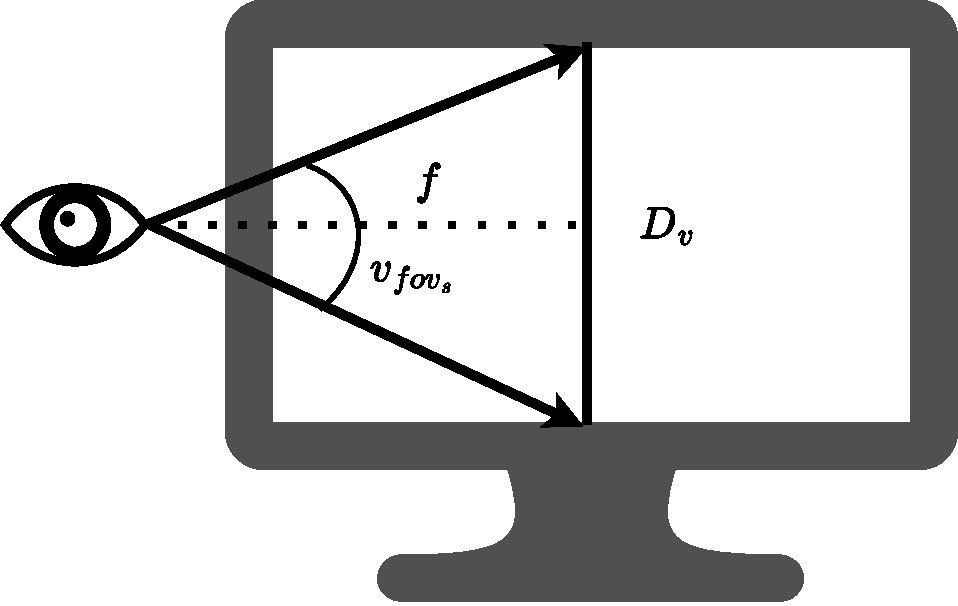
\includegraphics[width=.52\columnwidth]{img/13_2.pdf}
  \label{taikan:kijuntods2}
  }
  \caption{基準視野角とその導出の諸条件}
  \label{taikan:kijuntods}
\end{center}
\end{figure}

\begin{align}
    h_{fov_s} = 2\arctan{\frac{D_h}{2f}} \label{taikan:eq:kijun1}\\
    v_{fov_s} = 2\arctan{\frac{D_v}{2f}} \label{taikan:eq:kijun2}
\end{align}

$h_{fov_s}$:基準水平視野角\si{[degree]}、$v_{fov_s}$:基準垂直視野角\si{[degree]}、$f$:視点距離\si{[cm]}とする。

次に、基準視野角を映像クロップによる視野角に変換する。クロップ率$n$の値域は、$1 \leqq n \leqq 3.5$とする。
$n = 1$の時$h_{fov_s}$、$v_{fov_s}$(基準視野角)とする。
式\eqref{taikan:eq:crop1}、\eqref{taikan:eq:crop2}は、映像のクロップにより、視野範囲が変わることを意味する。
クロップは縦横比を一定とし、映像の中心は変化させない。図\ref{taikan:shiyatocrop}に映像クロップによる視野角とその導出の諸条件を示す。
\clearpage
\begin{figure}[h]
  \begin{center}
  \subfigure[水平方向]{
  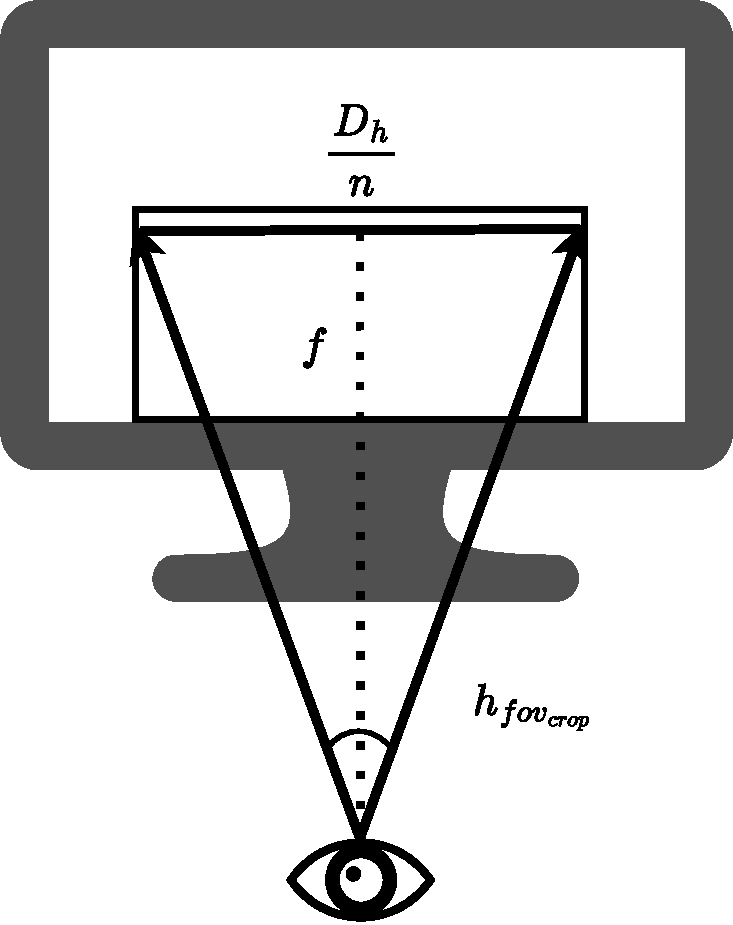
\includegraphics[width=.4\columnwidth]{img/14_1.pdf}
  \label{taikan:shiyatocrop1}
  }
  \subfigure[垂直方向]{
  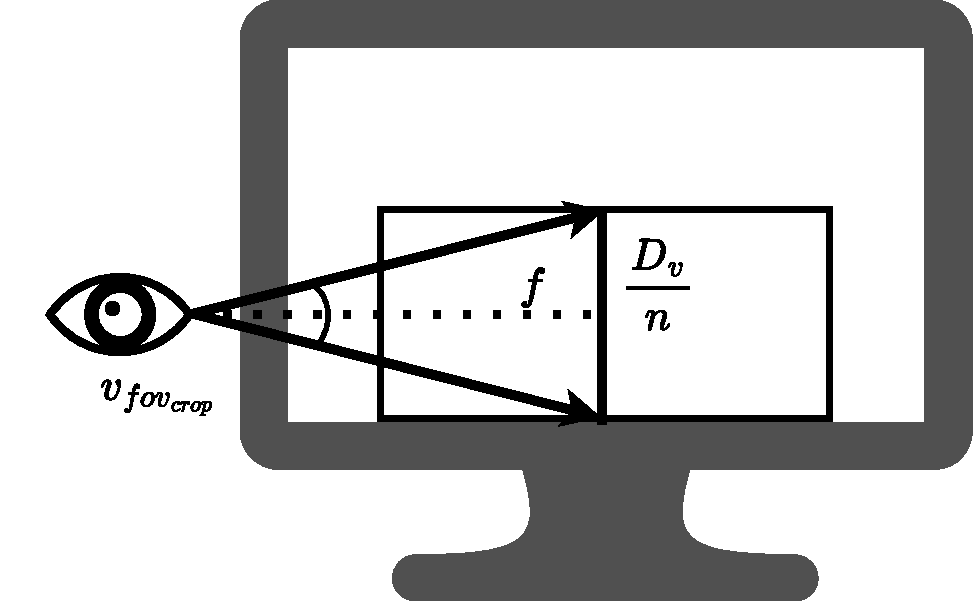
\includegraphics[width=.52\columnwidth]{img/14_2.pdf}
  \label{taikan:shiyatocrop2}
  }
  \caption{映像クロップによる視野角とその導出の諸条件}
  \label{taikan:shiyatocrop}
  \end{center}
\end{figure}

\begin{align}
  h_{fov_{crop}} = 2\arctan{\frac{D_h}{2f\cdot n}} \label{taikan:eq:crop1}\\
  v_{fov_{crop}} = 2\arctan{\frac{D_v}{2f\cdot n}} \label{taikan:eq:crop2}
\end{align}

$h_{fov_{crop}}$:映像クロップによる水平視野角\si{[degree]}、$v_{fov_{crop}}$:映像クロップによる垂直視野角\si{[degree]}、$n$:クロップ率の関数

次に、変数の視野角を基準よりも大きくとる場合に拡張する。つまり、$n<1$を考える。$n = 0.2 \thicksim 1$として拡張し、得られた視野角を変数
$h_{fov_v}$、$v_{fov_v}$とおく、これを体感速度のパラメータとする。$n$は、クロップ率を基準視野角から拡大または縮小するための値として拡張した、視野角拡大率とする。
$n$は、$h_{fov_v}$、$v_{fov_v}$のパラメータである。つまり、体感速度$v_{sense} = f(h_{fov_v}) = f(g(n))$とし、$h_{fov_v}=g(n)$である。
これらの式を、式\eqref{taikan:eq:kakudai1}、\eqref{taikan:eq:kakudai2}に示す。

\begin{align}
  h_{fov_v} = 2\arctan{\frac{D_h}{2f\cdot n}} \label{taikan:eq:kakudai1}\\
  v_{fov_v} = 2\arctan{\frac{D_v}{2f\cdot n}} \label{taikan:eq:kakudai2}
\end{align}

$h_{fov_v}$:水平視野角変数\si{[degree]}、$v_{fov_v}$:垂直視野角変数\si{[degree]}、$n$:視野角拡大率とする。

次に、体感速度は、基準視野角と水平視野角変数におけるそれぞれの映像のポール間ピクセル数の比を、実速度に乗ずることで式\eqref{taikan:eq:vsense}により求められる。

\begin{align}
  v_{sense} = \frac{px_v}{px_s}v_s = m_{sense}\cdot v_s \label{taikan:eq:vsense}
\end{align}

$px_v$:$h_{fov_v}$におけるポール間ピクセル数\si{[px]} (実測値)、$px_s$:$h_{fov_s}$におけるポール間ピクセル数\si{[px]}実測値、$v_{sense}$:体感速度\si{[km/h]}、$v_s$:実速度\si{[km/h]}、$m_{sense}$:ポール間ピクセル数の比とする。

図\ref{taikan:px}に視野角の違いによるポール間ピクセル数の違いを示す。

\begin{figure}[h]
  \begin{center}
  \subfigure[基準視野角]{
  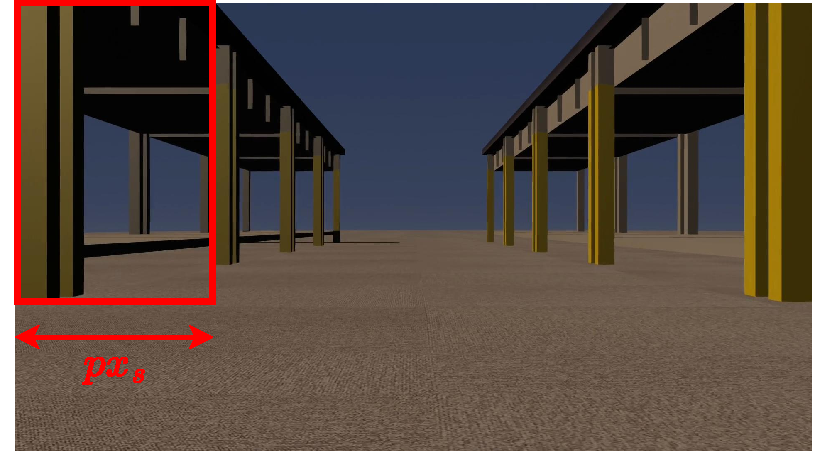
\includegraphics[width=.8\columnwidth]{img/15_1.pdf}
  \label{taikan:pxs}
  }
  \subfigure[変化視野角(増加)]{
  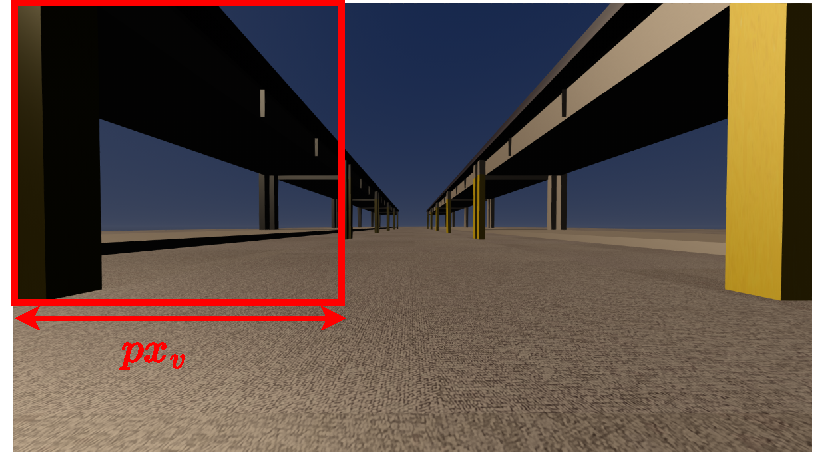
\includegraphics[width=.8\columnwidth]{img/15_2.pdf}
  \label{taikan:pxv}
  }
  \caption{視野角の違いによるポール間ピクセル数の違い}
  \label{taikan:px}
  \end{center}
\end{figure}

次に、$v_{sense}=f(h_{fov_v})$となる$f$を導きたい。$v_s$は一定として考えているため、$m_{sense}=f(h_{fov_v})$を導く。ここで、
視野角変数$h_{fov_v}$において、映像中のボールが画面の端にあるとする。(視点とディスプレイの短辺は$h_{fov_v}$の角度をなす。)
そこから、次のボールが画面の端になるように縦横比一定でクロップした時のクロップ率を視野辺ピクセル倍率$n_{p_{\to}p}$とする。
基準視野角においても同様に、$n_{p_{\to}p_s}$(基準視野角の場合の$n_{p_{\to}p_s}$)を求める。なお、遠近法より、$n_{p_{\to}p_s} = 2$であることが一般的に知られている。すると、
$m_{sense}$は、図\ref{taikan:kika}に示す視野角に関する幾何学を用いて、
式\eqref{taikan:eq:kika1}\verb|~|\eqref{taikan:eq:kika3}のように求めることができる。

\begin{figure}[h]
  \begin{center}
  \subfigure[基準視野角の幾何学]{
  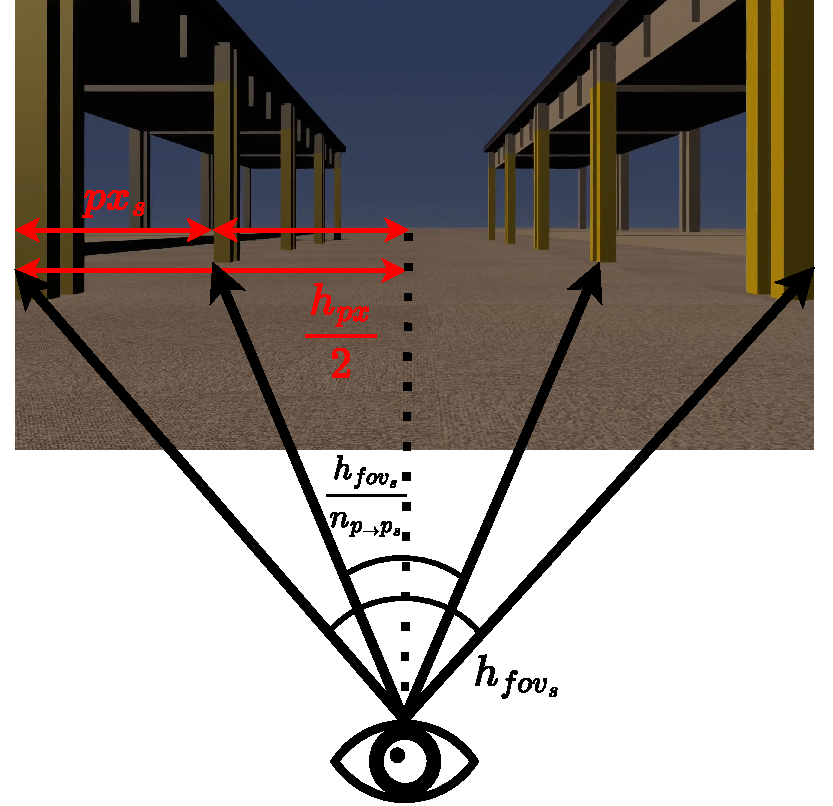
\includegraphics[width=.45\columnwidth]{img/16_2.pdf}
  \label{taikan:kika1}
  }
  \subfigure[変化視野角の幾何学]{
  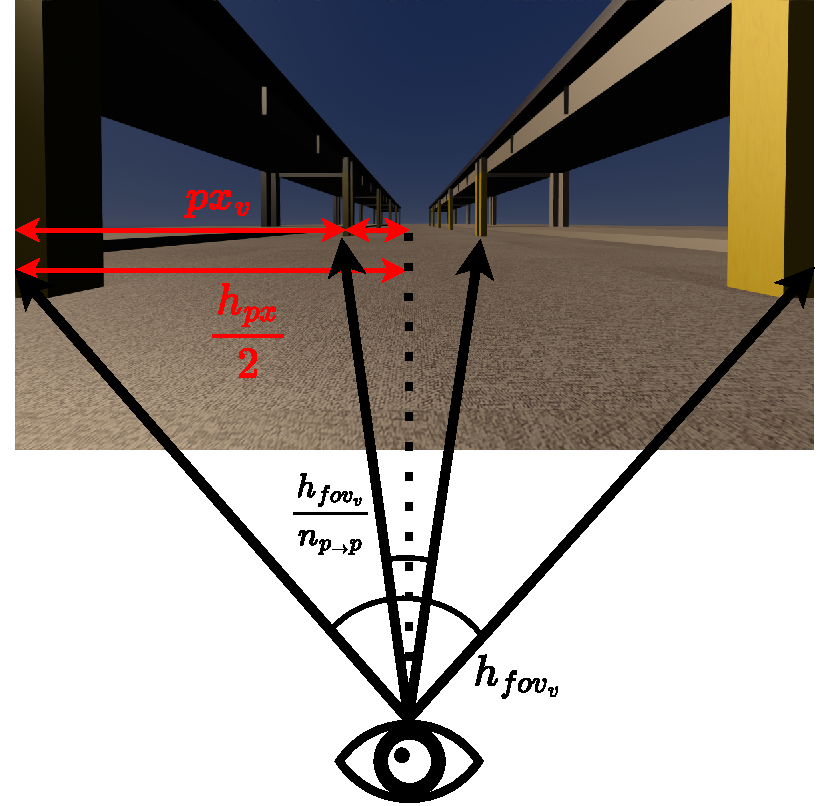
\includegraphics[width=.45\columnwidth]{img/16_3.pdf}
  \label{taikan:kika2}
  }
  \subfigure[$n_{p_{\to}p}$について]{
  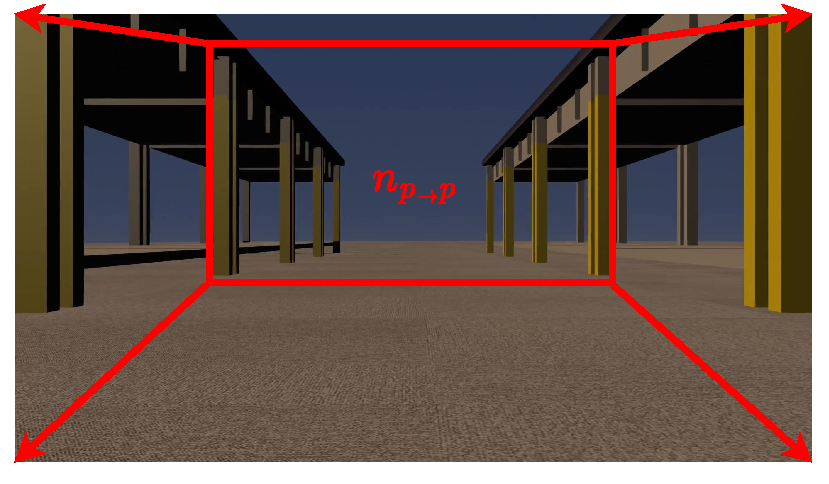
\includegraphics[width=.45\columnwidth]{img/16_1.pdf}
  \label{taikan:kika3}
  }
  \caption{視野角に関する幾何学}
  \label{taikan:kika}
  \end{center}
\end{figure}

\begin{align}
  px_s &= \frac{h_{px}}{2} - \frac{h_{px}}{2}\Bigg(\frac{\tan\frac{h_{fov_s}}{2\cdot n_{p_{\to}p_s}}}{\tan{\frac{h_{fov_s}}{2}}}\Bigg) = \frac{h_{px}}{2}\Biggl(1-\frac{\tan{\frac{h_{fov_s}}{4}}}{\tan{\frac{h_{fov_s}}{2}}}\Biggr) \label{taikan:eq:kika1}\\
  px_v &= \frac{h_{px}}{2} - \frac{h_{px}}{2}\Bigg(\frac{\tan\frac{h_{fov_v}}{2\cdot n_{p_{\to}p_v}}}{\tan{\frac{h_{fov_v}}{2}}}\Bigg) = \frac{h_{px}}{2}\Biggl(1-\frac{\tan{\frac{h_{fov_v}}{2\cdot n_{p_{\to}p}}}}{\tan{\frac{h_{fov_v}}{2}}}\Biggr) \label{taikan:eq:kika2}\\
  m_{sense} &= \frac{px_v}{px_s} = \frac{\Biggl\{\frac{h_{px}}{2}\Bigg(1-\frac{\tan\frac{h_{fov_v}}{2\cdot n_{p_{\to}p}}}{\tan\frac{h_{fov_v}}{2}}\Bigg)\Biggr\}}{\Biggl\{\frac{h_{px}}{2}\Bigg(1-\frac{\tan\frac{h_{fov_s}}{4}}{\tan\frac{h_{fov_s}}{2}}\Bigg)\Biggr\}} = \frac{1-\frac{\tan\frac{h_{fov_v}}{2\cdot n_{p_{\to}p}}}{\tan\frac{h_{fov_s}}{2}}}{1-\frac{\tan\frac{h_{fov_s}}{4}}{\tan\frac{h_{fov_s}}{2}}} = f(h_{fov_v}) \label{taikan:eq:kika3}
\end{align}

$h_{px}$:ディスプレイの横のピクセル比\si{[px]}(1920 \si{[px]})、$n_{p_{\to}p}$:$h_{fov_v}$における視野辺ピクセル倍率(実測値)、
$n_{p_{\to}p_s}$:$h_{fov_s}$における視野辺ピクセル倍率(定数値:2)。

ここで、幾何学的に求められた$f(m_{sense})$を、体感速度$v_{sense}$の理論式とする。$h_{fov_v}$を$v_{sense}$に変換する。式\eqref{taikan:eq:kika3}を整理すると、
式\eqref{taikan:eq:final}のようになる。

\begin{equation}
  \begin{split}
    m_{sense} &= \frac{px_v}{px_s} = \frac{1-\frac{\tan\frac{h_{fov_v}}{2\cdot n_{p_{\to}p}}}{\tan\frac{h_{fov_v}}{2}}}{1-\frac{\tan\frac{h_{fov_s}}{2\cdot n_{p_{\to}p_s}}}{\tan\frac{h_{fov_s}}{2}}} = \frac{1-\frac{\tan\frac{h_{fov_v}}{2\cdot n_{p_{\to}p}}}{\tan\frac{h_{fov_v}}{2}}}{1-\frac{\tan\frac{28}{2\cdot 1.986}}{\tan\frac{28}{2}}}=1.923\cdot \Bigg(1 - \frac{\tan\frac{h_{fov_v}}{2\cdot n_{p_{\to}p}}}{\tan\frac{h_{fov_v}}{2}}\Bigg)\\ \label{taikan:eq:final}
    &= f(h_{fov_v}, n_{p_{\to}p}) = 1.923\cdot \Bigg(1 - \frac{\tan\frac{h_{fov_v}}{2\cdot 1.078415307\cdot e^{0.011995591\cdot h_{fov_v}}}}{\tan\frac{h_{fov_v}}{2}}\Bigg) = f(h_{fov_v})
  \end{split}
\end{equation}

よって、式\eqref{taikan:eq:final}は、式\eqref{taikan:eq:sensefinal}のようになる。

\begin{align}
  v_{sense} = 19.30\Bigg(1-\frac{\tan\frac{h_{fov_v}}{2\cdot 1.078415307\cdot e^{0.011995591\cdot h_{fov_v}}}}{\tan\frac{h_{fov_v}}{2}}\Bigg) \label{taikan:eq:sensefinal}
\end{align}

$n_{p_{\to}p}$は、式\eqref{taikan:eq:kaiki}による回帰曲線とした。

\begin{align}
  n_{p_{\to}p} = 1.078415307\cdot e^{0.011995591\cdot h_{fov_v}} \label{taikan:eq:kaiki}
\end{align}

この式を基準視野角における倍率をクロップ倍率を$m$として、正規化すると、式\eqref{taikan:eq:mseiki}

\begin{align}
  m_{sense} = \frac{px_v}{px_s} = \frac{1-\frac{\tan\frac{h_{fov_v}}{2\cdot p_{p_{\to}p}}}{\tan\frac{h_{fov_v}}{2}}}{1-\frac{\tan\frac{h_{fov_s}}{2\cdot n_{p_{\to}p_s}}}{\tan\frac{h_{fov_s}}{2}}} = \frac{1-\frac{\tan\frac{h_{fov_v}}{2\cdot n_{p_{\to}p}}}{\tan\frac{h_{fov_s}}{2}}}{1-\frac{\tan\frac{h_{fov_s}}{2\cdot 1.986}}{\tan\frac{h_{fov_s}}{2}}} = \frac{1-\frac{\tan\frac{h_{fov_v}}{2\cdot n_{p_{\to}p}}}{\tan\frac{h_{fov_v}}{2}}}{1-\frac{\tan\frac{h_{fov_s}}{2\cdot 1.986\cdot m}}{\tan\frac{h_{fov_s}}{2}}} \label{taikan:eq:mseiki}
\end{align}
$$m=1/1.986$$

よって、以上をまとめると、式\eqref{taikan:eq:v}、\eqref{taikan:eq:fov}となる。

\begin{align}
  v_{sense} &= 19.30\cdot\Bigg(1-\frac{\tan\frac{h_{fov_v}}{2\cdot n_{p_{\to}p}}}{\tan\frac{h_{fov_v}}{2}}\Bigg) = f(h_{fov_v})\cdot v_s = f(g(n))\cdot v_s \label{taikan:eq:v}
\end{align}
\begin{align}
  h_{fov_v} &= 2\arctan\frac{D_h}{2f\cdot n} \label{taikan:eq:fov}
\end{align}

以上により、視野角、クロップ率を体感速度の倍率に変換する以下の式を導いた。
\begin{align*}
  v_{sense} = f(h_{fov_v})\cdot v_s = f(g(n))\cdot v_s
\end{align*}
\begin{align*}
  h_{fov_v} = g(n)
\end{align*}

この定式モデルを用いることで、基準視野角に対して、任意の視野角における体感速度を求めることができる。
また、視野角はクロップ率の関数であるため、任意のクロップ率に対しての体感速度を求めることもできる。
この定式モデルでは、パラメータを視野角としたが、その他にも、体感速度を決める環境のパラメータとして、ディスプレイ長さや、
インチ数等も用いることができる。したがって、走行映像の取得環境に応じた変数と固定値を入れ替えることで、あらゆる環境の幾何学的なパラメータに対応した定式モデルと言える。
このモデルの大まかな特性を求めるために、$m_{sense}$を累乗で近似すると、式\eqref{taikan:eq:shijo}となり、
体感速度は、式\eqref{taikan:eq:shijov}で表すことができる。

\begin{align}
  m_{sense} = 0.086537715\cdot h_{fov_v}^{0.615630604} \label{taikan:eq:shijo}\\
  v_{sense} = 0.86537715\cdot h_{fov_v}^{0.615630604} \label{taikan:eq:shijov}
\end{align}

従って、$v_{sense}$は、視野角の$n$乗根に比例する軌跡となる。その概形は、緩やかに上昇する軌跡である。

\section{提案モデルの検証実験}
これまで、体感速度の定式化を提案した。ここでは、提案したモデルが正しいことを実証するための検証実験に関して述べる。
前述の体感速度のモデルを実証するために、以下の手順で実験を行った。

\subsection{定式化モデルと実測値の比較}
前と同様のRCカーの走行環境を模したDS走行環境において走行実験を行う。基準視野角における速度と映像のクロップ率を変化させた時の体感速度との比率をポール間ピクセル数の計測により求める。
ポール間をディスプレイの横幅まで拡大し、ディスプレイの解像度をその拡大倍率で割ることでポール間ピクセル数が導出される。
今回、定式化したモデルは、水平視野角をパラメータとして用いているが、
DS環境設定では、垂直視野角を設定値とする仕様であるため、水平視野角を垂直視野角に変換した値をDS環境の視野角設定に用いる。
基準視野角(垂直視野)を20度として、DS環境設定の視野角変更機能により、視野角を変化させる。
図\ref{taikan:shiyaset}にDSの視野角設定を示す。

\begin{figure}[h]
  \begin{center}
  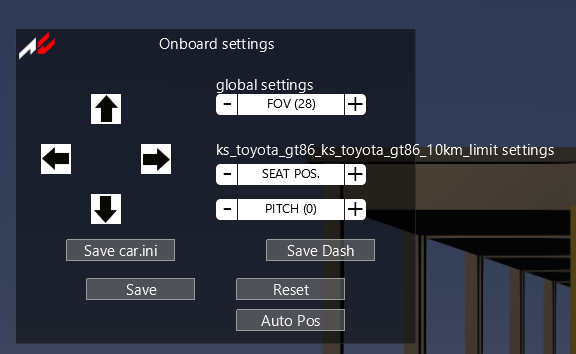
\includegraphics[width=.65\linewidth]{img/17.png}
  \caption{DSの視野角設定}
  \label{taikan:shiyaset}
  \end{center}
\end{figure}

DS乗で定速走行した映像を解析し、基準視野角とポール間ピクセル数を実測する。基準視野角と、ある視野角の関係から幾何学的にポール間ピクセル数を計算し、定速度値に乗じることで体感速度を実測する。
幾何学的な倍率は一部実測値を含む。その後、実測値と幾何学モデルとの一部実測値を含む。実測値と幾何学モデルとの一致を確認する。基準視野角で実速度10 \si{[km/h]}、体感速度10 \si{[km/h]}の映像と、
ある視野角を変えて実速度10 \si{[km/h]}、体感速度17 \si{[km/h]}(単位時間のポール間の移動ピクセル数が1.7倍になったもの)の映像と、基準視野角で実測度17 \si{[km/h]}、体感速度17 \si{[km/h]}、体感速度17 \si{[km/h]}
(単位時間に通過する柱の数が1.7倍になったもの)の映像を比較して、この仮説を検証する。

\begin{figure}[h]
  \begin{center}
  \subfigure[基準視野角]{
  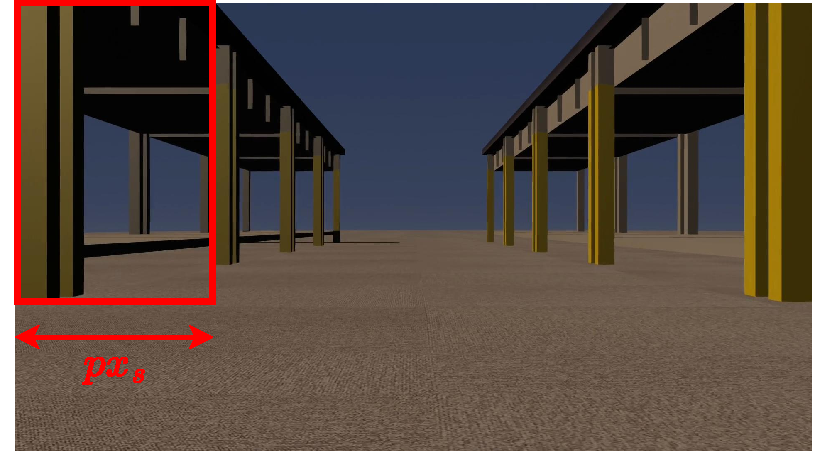
\includegraphics[width=.45\columnwidth]{img/17_1.pdf}
  \label{taikan:pxs_1}
  }
  \subfigure[変化視野角(増加)]{
  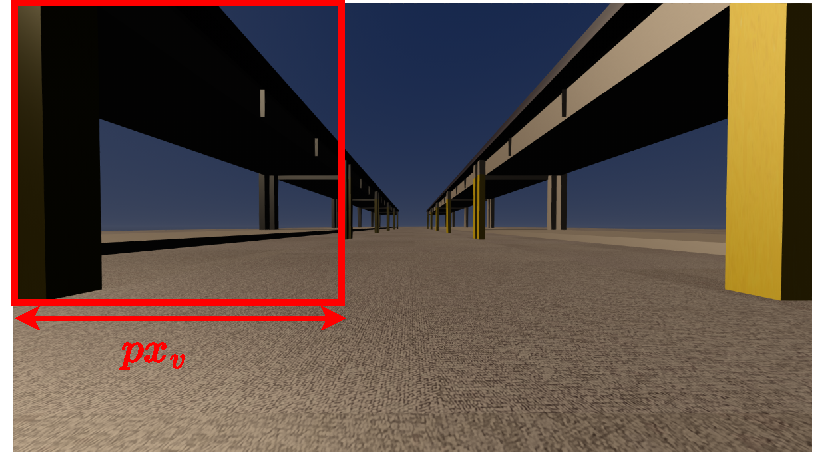
\includegraphics[width=.45\columnwidth]{img/17_2.pdf}
  \label{taikan:pxv_1}
  }
  \subfigure[変化視野角(増加)]{
  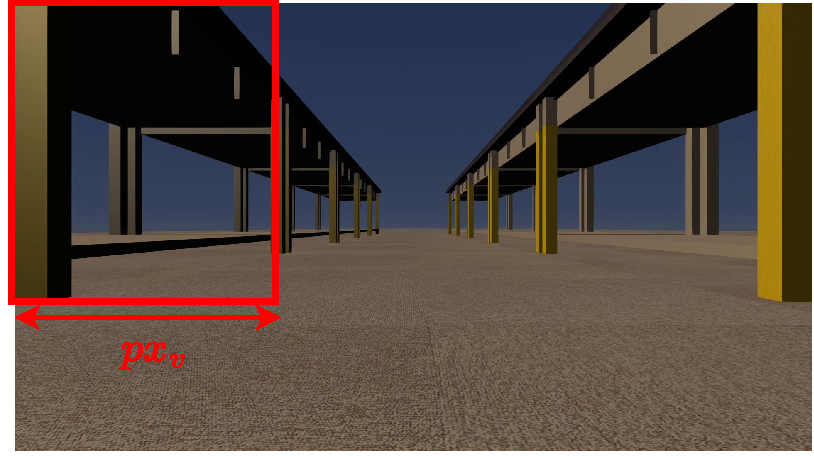
\includegraphics[width=.45\columnwidth]{img/17_3.pdf}
  \label{taikan:pxv_2}
  }
  \caption{視野角の違いによるポール間ピクセル数の違い}
  \label{taikan:px_sv}
  \end{center}
\end{figure}

一例として、基準視野角に対する視野角での見え方を図\ref{taikan:px_sv}に示す。赤線の横辺のピクセル数を求める。

\subsection{実験条件}
今回の実験で用いた環境と実験条件を示す。本研究で定式化したモデルは、水平視野角をパラメータとして用いているが、DS環境設定では、垂直視野角を設定値とする仕様であるため、水平視野角を垂直視野角に変換した値をDS環境の視野角設定に用いる。
その指定値を$v_{fov}$と、cropとして、表\ref{taikan:table2}に示す。本研究では、クロップ率をパラメータとして定めると、$v_{fov_v}$を求めることができるため、クロップ率cropに対応する視野角を用いる。

\begin{table}[h]
  \centering
  \caption{水平視野角の指定値$v_{fov}$とクロップ率cropとの対応}
  \scalebox{.6}{
  \begin{tabular}[t]{rrrrrrrrrrrrrrrrrrrrrrrrr}
  \toprule
  $v_{fov}$\si{[degree]}:&8&9&10&11&12&13&14&15&16&17&19&20&21&23&25&28&30&34&39&44&52&63&78&102\\
  \midrule
  crop:&0.2&0.3&0.4&0.5&0.6&0.7&0.8&0.9&1.0&1.1&1.2&1.3&1.4&1.5&1.6&1.7&1.8&2&2.2&2.4&2.6&2.8&3.1&3.5\\
  \bottomrule
  \label{taikan:table2}
  \end{tabular}}
\end{table}%

また、本実験で使用した環境について表\ref{taikan:table3}に示す。

\begin{table}[h]
  \centering
  \caption{本研究で使用した環境}
  \scalebox{.8}{
  \begin{tabular}[t]{c}
    \toprule
    環境\\
    DS:Asetto Corsa 1.16\\
    ディスプレイ:iiyama ProLite P2474HS 23.6インチ full HD 1920x1080 60 Hz\\
    MOD:ACContentManager 0.8.2569.39678\\
    カメラ:gopro hero8\\
    CGソフト:Blender\\
    \bottomrule
    \label{taikan:table3}
  \end{tabular}}
\end{table}

\subsection{定式化モデルの検証方法}
DS走行環境においてピクセル倍率を実測する。まず、動画編集ソフトを用いて、映像中のポール間距離を画面上の左右のサイズになるように拡大し、
左右のサイズを拡大率で割ることで、走行映像におけるポール間ピクセル数$n_{p_{\to}p}$を求める。これを基準視野角と視野角を変化させた時で測定し、
基準視野角に対する、ある視野角でのピクセル数の比を求めて、体感速度比とする。次に、体感速度比と実際の速度を掛けて体感速度を導出する。
以上の手順で体感速度を求めて、視野角との特性をグラフ上にプロットする。定式モデルに、実験条件で示した視野角と先に求めた拡大率を代入し、体感速度を導出する。
定式モデルの視野角と体感速度の特性をグラフ上にプロットする。定式モデルでの拡大率は、視野角の変数で表すことが困難であるため、実測値を用いる。

\subsection{体感速度を変化させる効果の検証}
定式化モデルが体感速度を変化させる効果を与えることの検証として、以下の手順を行う。
\begin{enumerate}
  \item 基準視野角(垂直28度)、実速度が基準速度と等しく10 \si{[km/h]}、体感速度が基準速度と等しい映像を取得する。
  \item ある視野角(垂直102度)、実速度10 \si{[km/h]}、体感速度17 \si{[km/h]}での走行映像を取得する。
  \item 基準視野角(垂直28度)、実速度17 \si{[km/h]}、体感速度17 \si{[km/h]}での走行映像を取得する。
  \item 基準視野角・実速度17 \si{[km/h]}、体感速度17 \si{[km/h]}の映像と、ある視野角(垂直102度)、実速度17 \si{[km/h]}、体感速度17 \si{[km/h]}(単位時間のポールの移動ピクセル数が1の時の1.7倍になったもの)の映像を取得する。
\end{enumerate}

\subsection{実験結果}

\subsubsection{定式化モデルと実測値の比較}
実験結果を図\ref{taikan:kekka1}、\ref{taikan:kekka2}に示す。

\begin{figure}[h]
  \begin{center}
  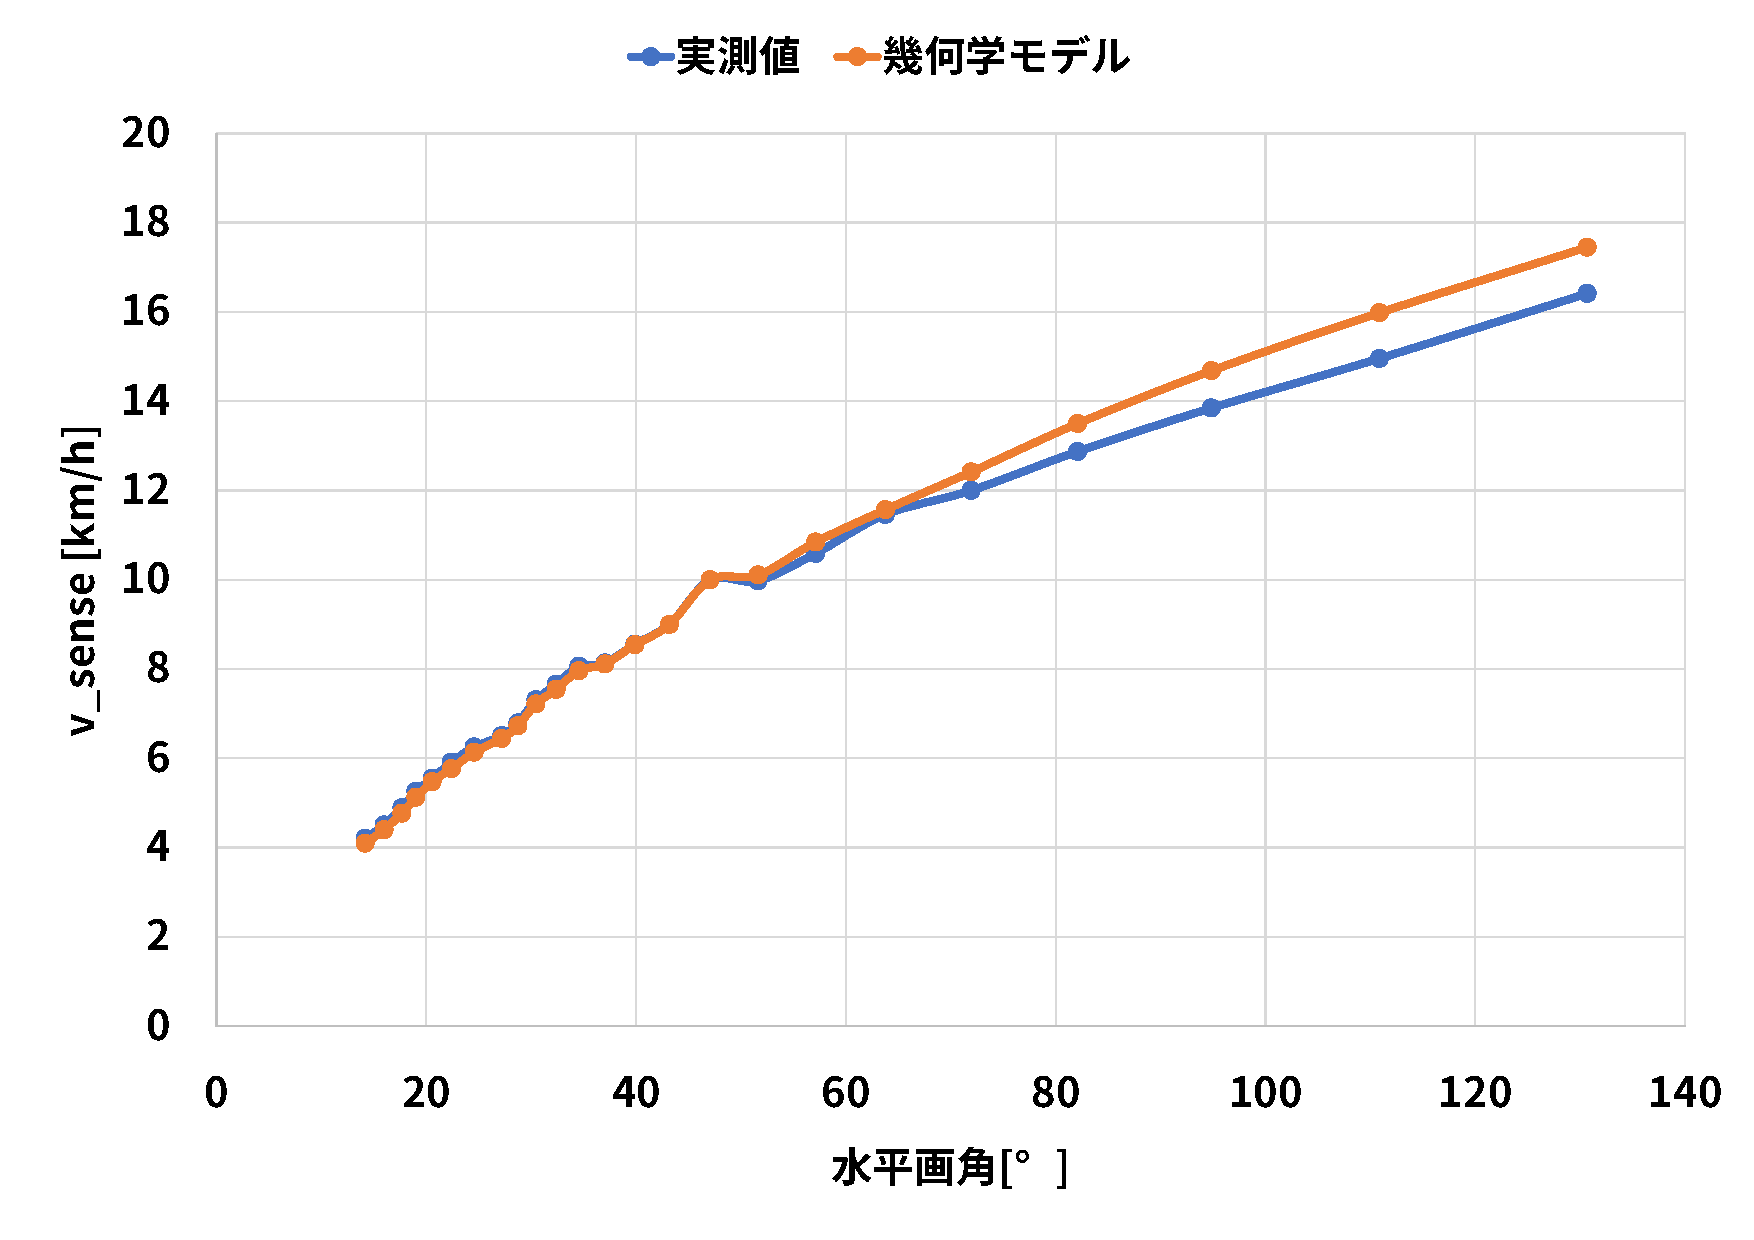
\includegraphics[width=.85\linewidth]{img/19.pdf}
  \caption{水平視野角と体感速度の特性}
  \label{taikan:kekka1}
  \end{center}
\end{figure}

幾何学モデルの理論式を式\eqref{taikan:eq:kekka1}\verb|~|\eqref{taikan:eq:kekka4}に示す。$n_{p_{\to}p}$は、実測である。

\begin{align}
  v_{sense} = 19.30\Bigg(1-\frac{\tan\frac{h_{fov_v}}{2\cdot n_{p_{\to}p}}}{\tan\frac{h_{fov_v}}{2}}\Bigg) \label{taikan:eq:kekka1}
\end{align}
\begin{align}
  h_{fov_v} = 2\arctan\Bigg(\frac{D_h}{2f\cdot n}\Bigg) \label{taikan:eq:kekka2}
\end{align}
\begin{align}
  n = \frac{D_h}{2f\tan\frac{h_{fov_v}}{2}} \label{taikan:eq:kekka3}
\end{align}
\begin{align}
  v_{fov_v} = 2\arctan\frac{D_v}{2f\cdot n} \label{taikan:eq:kekka4}
\end{align}

以上の式\eqref{taikan:eq:kekka5}、\eqref{taikan:eq:kekka6}を用いて、$v_{fov_v}$を、$h_{fov_v}$に変換し、$h_{fov_v}$を変数とする。

\begin{align}
  h_{fov_v} = 2\arctan\frac{D_h}{2f\cdot n} \label{taikan:eq:kekka5}
\end{align}
\begin{align}
  v_{sense} = 19.30\cdot \Bigg(1-\frac{\tan\frac{h_{fov_v}}{2\cdot n_{p_{\to}p}}}{\tan{\frac{h_{fov_v}}{2}}}\Bigg) \label{taikan:eq:kekka6}
\end{align}

\begin{figure}[h]
  \begin{center}
  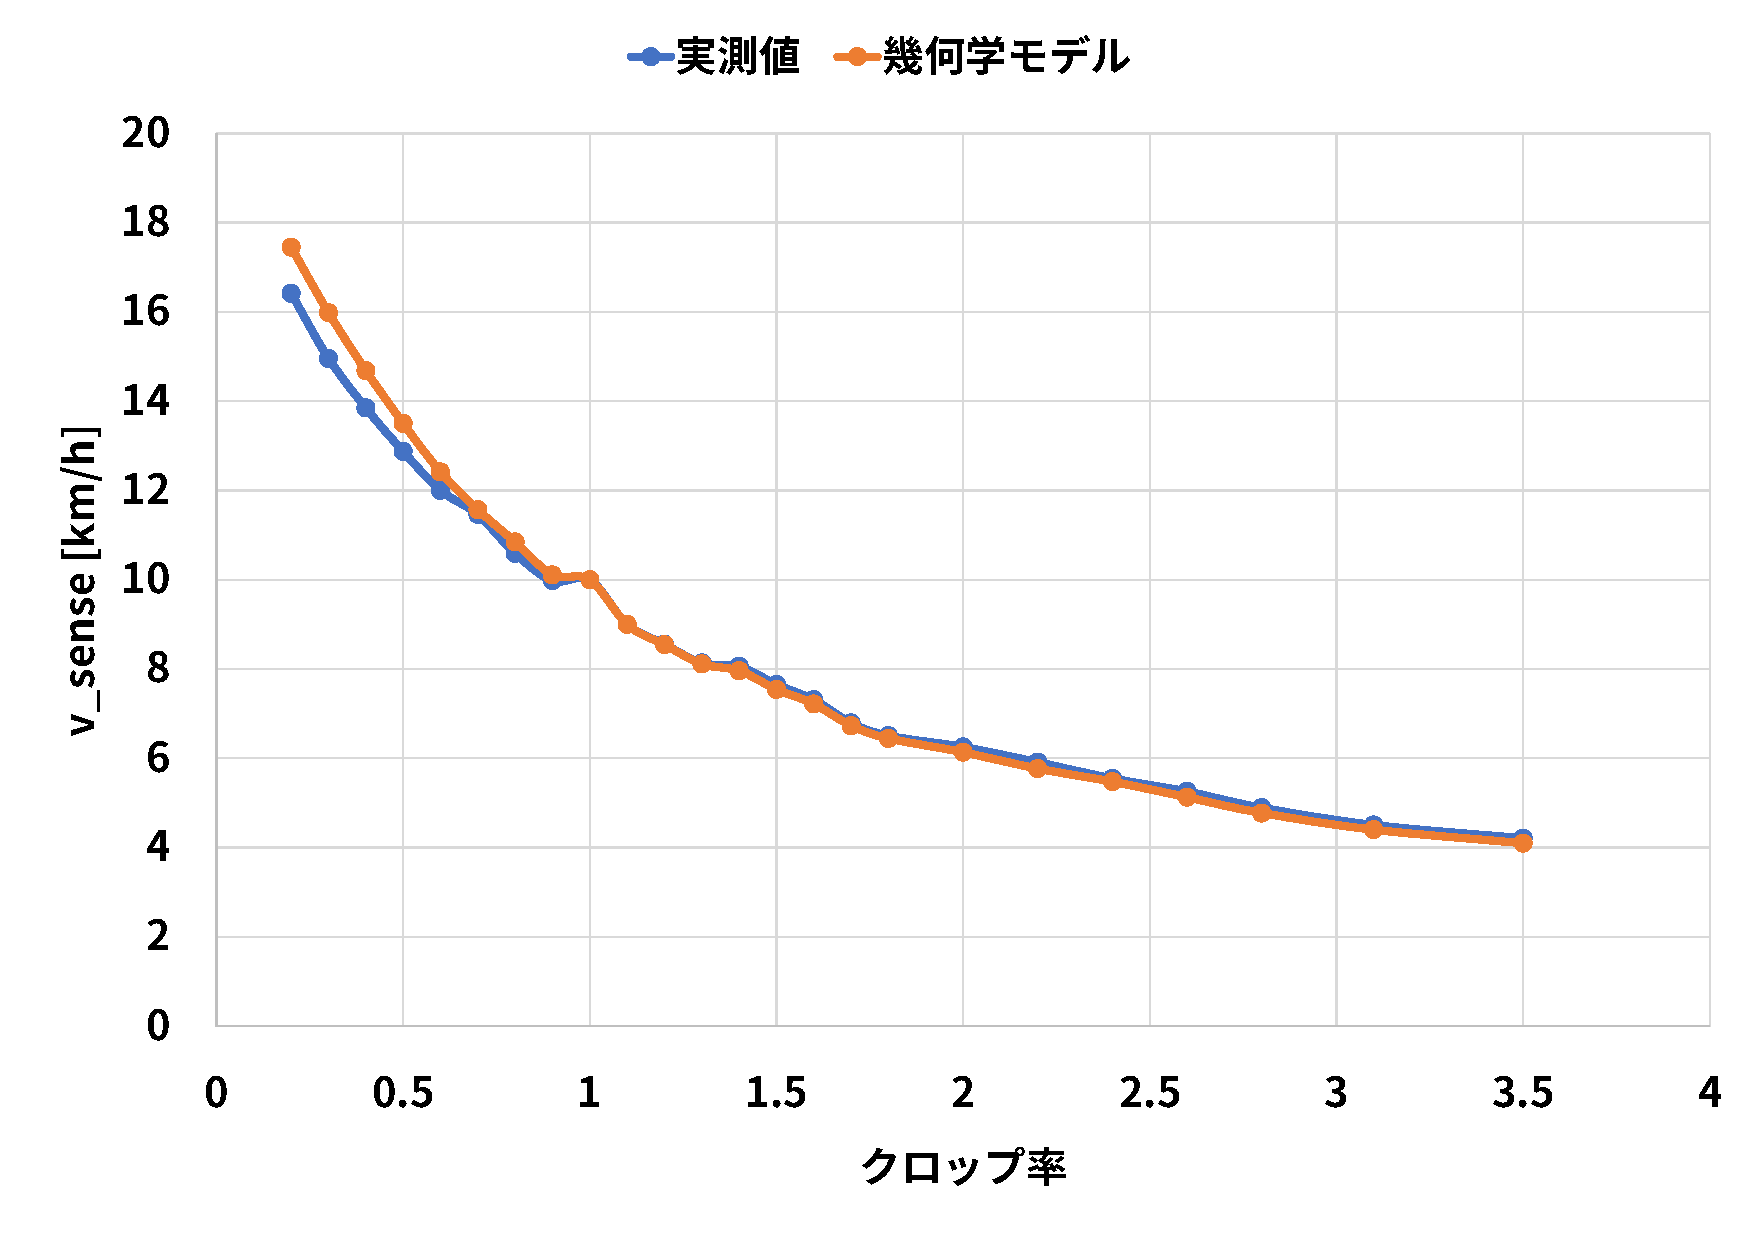
\includegraphics[width=.85\linewidth]{img/20.pdf}
  \caption{クロップ率と体感速度の特性}
  \label{taikan:kekka2}
  \end{center}
\end{figure}

\clearpage

\subsubsection{体感速度を変化させる効果の検証}
実験結果を以下に示す。
\begin{enumerate}
  \item ピクセル比と実速度比の一致の確認\\
  基準視野角(垂直28度)、実速度が基準速度と等しく10 \si{[km/h]}、体感速度が基準速度と等しい映像に関して\\
  ポール間移動時間:5.25秒、ポール間ピクセル数:480 \si{[px]}\\
  ある視野角(垂直120度)、実速度10 \si{[km/h]}、体感速度17 \si{[km/h]}での走行映像に関して\\
  ポール間移動時間:5.25秒、ポール間ピクセル数:788 \si{[px]}\\
  時間比:$5.5\div 3.05 = 1.7213$\\
  ピクセル比:$788\div 480 = 1.64$\\
  体感速度:時間比$\times 10 = 17.213 = 17$ \si{[km/h]}\\
  誤差:$\frac{17.2-16.4}{16.4}\times 100 = 4.878 = 4.9$ \%
  \item 体感速度比(時間比)とピクセル比の一致の確認\\
  ある視野角(垂直102度)、実速度10 \si{[km/h]}、体感速度17 \si{[km/h]}での走行映像に関して、\\
  ポール間移動距離:5.25秒、ポール間ピクセル数:788 \si{[px]}\\
  基準視野角(垂直28度)、実速度17 \si{[km/h]}、体感速度17 \si{[km/h]}での走行映像に関して\\
  ポール間移動距離:2.96秒、ポール間ピクセル数:463 \si{[px]}\\
  時間比:$5.25\div 2.96 = 1.7736$\\
  ピクセル比:$788\div 463 = 1.7019$\\
  体感速度:$1.7736\times 10 = 17.7$ \si{[km/h]}\\
  誤差:$(1.7736-1.7019)\div 1.7019 \times 100 = 4.2129 = 4.2$\%
\end{enumerate}
よって、これらの定式化が実測と同程度であることを確認した。

\section{考察}
\subsection{定式化モデルと実測値の比較に関して}
視野角-体感速度特性において、視野角の増加に伴って体感速度は緩やかに増加する。
この結果は定説と一致している。特性の概形は、おおよそ視野角の$n$乗根に比例すると考えられる点が仮定と一致していた。
基準視野角よりも小さな視野角値である時は、比例的に増加するが、基準視野角以上の値をとると、理論値、実測値ともに体感速度の変化率は緩やかになる。
また、視野角が70度以上の値をとると、理論値と、理論値との差が大きくなる。視野角が基準視野角よりも大きな値である映像は、基準視野角よりも小さな視野角の映像と比べて、映像の奥行きが大きくなり、映像自体が歪んでいることが分かる。
このことから、定式化モデルとして、ひずみに関するパラメータを考慮する必要があることが分かる。
なお、今回の定式化モデルでは、理想的な2次元の映像として考えていたため、このひずみに関しては考慮していない。考慮するためには、3次元の立体映像に関する知見が必要である。
クロップ率-体感速度特性について、クロップ率の増加に伴い体感速度は急激に減少する。
クロップ率を増加させると視野角が減少するため、視野角の減少により体感速度が減少することが定説通りであることを確認した。
クロップ率が1よりも大きな値をとる場合は、視野角を増加させていることと考えると、先に述べた点と一致している。

\subsection{体感速度を変化させる効果の検証}
ピクセル比と実速度比の一致の確認に関して、時間比と速度比は、定義通り一致していたが、単位時間当たりの移動ピクセル数と実速度比に関しては、4.9 \% 程の誤差がみられた。
DSでは小数点以下の速度は表示されないため、この誤差は、DS上における実速度の誤差であると考えられる。
このことから、体感速度に関する仮説として、視野角の変化によって、走行映像中のポール間ピクセル数が変化していることが体感速度の変化を表していることが実証された。
体感速度比とピクセル比の一致に関して、視野角をパラメータとして求めた体感速度と、その体感速度値と一致する実速度の映像では、単位時間当たりに進行するピクセルの比率がほとんど一致するため、単位時間当たりに移動するポール数は一致しないが、単位時間当たりに進行するピクセル数が一致することが確認された。
この結果より、体感速度を支配するパラメータとして提案されていた、映像中の風景線が流れるスピードが一致していることが分かる。
また検証により、視野角やクロップ率をパラメータとして、幾何学的に単位時間当たりに移動するピクセル比を導出する手法を用いた体感速度のモデルが正しいことが明らかになった。

\section{おわりに}
本章では、走行映像における体感速度を支配するパラメータを明らかにし、そのパラメータを用いて、体感速度の変化率のモデルを定量化した。
映像のクロップ率と映像の視野角(撮影画角) が最も影響力の大きいパラメータであることが明らかになった。
体感速度のモデルとして、映像の視聴環境とクロップ率と視野角を用いて幾何学的な計算によって導出したモデル(幾何学モデル)を提案した。
幾何学モデルが正しいことを検証するために、移動ピクセル数の実測値との比較により、検証実験により、実速度が異なる映像でも、体感速度が一致する視野角を設定することで、
単位時間当たりの移動ピクセル数が一致し、映像中の風景線が流れるスピードが一致したことから、幾何学モデルが正しいことを明らかにした。
提案した幾何学モデルに一部実測値を用いている点や、視野角を大きくしたときに生じた立体的なひずみが生じることが明らかになり、立体視野角を考慮した幾何学が必要であることに関して、
新たな知見を得た。この知見を基にモデルの改良に関する検討の余地があり、今後の課題とする。
本研究は、人間の視野が走行映像全体に均一に焦点しているという仮定の上で行っていた。今後は、人間の集中点・集中視野によって変化する体感速度のモデルに関して研究を行う予定である。
